\documentclass[tikz,border=5pt]{standalone}
\usepackage{tikz}
\usetikzlibrary{shapes,arrows,positioning,fit,calc}

\begin{document}
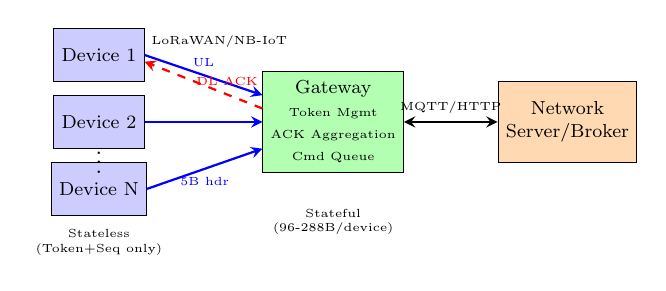
\begin{tikzpicture}[scale=0.85, transform shape,
    device/.style={rectangle, draw, fill=blue!20, minimum width=1.2cm, minimum height=0.8cm, font=\footnotesize},
    gateway/.style={rectangle, draw, fill=green!30, minimum width=2cm, minimum height=1.5cm, font=\footnotesize},
    server/.style={rectangle, draw, fill=orange!30, minimum width=2cm, minimum height=1.2cm, font=\footnotesize},
    arrow/.style={->, >=stealth, thick}
]
% Devices
\node[device] (d1) at (0,2) {Device 1};
\node[device] (d2) at (0,1) {Device 2};
\node[device] (d3) at (0,0) {Device N};
\node at (0,0.5) {$\vdots$};

% Gateway
\node[gateway, align=center] (gw) at (3.5,1) {Gateway\\\tiny Token Mgmt\\\tiny ACK Aggregation\\\tiny Cmd Queue};

% Server
\node[server, align=center] (srv) at (7,1) {Network\\Server/Broker};

% Arrows - Uplink
\draw[arrow, blue] (d1.east) -- node[above, font=\tiny] {UL} ($(gw.west)+(0,0.4)$);
\draw[arrow, blue] (d2.east) -- (gw.west);
\draw[arrow, blue] (d3.east) -- node[below, font=\tiny] {5B hdr} ($(gw.west)+(0,-0.4)$);

% Arrows - Downlink
\draw[arrow, red, dashed] ($(gw.west)+(0,0.2)$) -- node[above, font=\tiny, pos=0.3] {DL ACK} ($(d1.east)+(0,-0.1)$);

% Gateway to Server
\draw[arrow, <->] (gw.east) -- node[above, font=\tiny] {MQTT/HTTP} (srv.west);

% Labels
\node[font=\tiny, align=center] at (0,-0.8) {Stateless\\(Token+Seq only)};
\node[font=\tiny, align=center] at (3.5,-0.5) {Stateful\\(96-288B/device)};
\node[font=\tiny, align=center] at (1.8,2.2) {LoRaWAN/NB-IoT};

\end{tikzpicture}
\end{document}
